\newcommand{\templatesdir}{../../../templates}
\newcommand{\template}{template-slides-est}
\input{\templatesdir/\template/template}

\title[Grafos]{Grafos}
\subtitle{Definições, implementação e algoritmos}

\immediate\write18{dots/compile.sh grafo1 0.8 > dots/grafo1.tex}
\immediate\write18{dots/compile.sh grafo2 0.8 > dots/grafo2.tex}
\immediate\write18{dots/compile.sh grafo3 1 > dots/grafo3.tex}
\immediate\write18{dots/compile.sh grafo4 1 > dots/grafo4.tex}

\begin{document}

\maketitle

\begin{frame}{Material de consulta}
	\textbf{Leitura obrigatória:}
	\begin{itemize}
		\item Capítulo 1 de~\cite{Goldbarg2AndGoldbarg2012} -- Conceitos básicos.
		\item Capítulo 3 de~\cite{KleinbergAndTardos2006} -- Grafos.
	\end{itemize}
	
	\bigskip
	
	\textbf{Leitura complementar:}
	\begin{itemize}
		\item Capítulo 14 de~\cite{GoodrichEtAl2014} -- Algoritmos em grafos.
		\item Capítulo 15 de~\cite{Preiss2001} -- Grafos e algoritmos em grafos.
	\end{itemize}
\end{frame}


\begin{frame}{Definições básicas}
	\framesubtitle{O que é um grafo?}
	
	\begin{itemize}
		\item Grafos modelam relacionamentos entre pares de objetos.
		\item {\color{magenta}Notação:} $G = (V, E)$
		\begin{itemize}
			\item $V$ é o conjunto de vértices/nodos (objetos).
			\item $E$ é o conjunto de arestas/arcos (relacionamentos).
			\begin{itemize}
				\item Uma aresta possui dois vértices terminais: $e = \{u, v\}$ com $u, v \in V$.
				\item Os vértices $u$ e $v$ são ditos vizinhos.
			\end{itemize}
			\item Tamanho do grafo: $n = |V|$ e $m = |E|$.
		\end{itemize}
		
		\pause
		\item {\color{magenta}Representação visual:}
	\end{itemize}
	
	\vspace{-12pt}

	\begin{columns}
		\begin{column}{0.35\textwidth}
		\begin{figure}		
			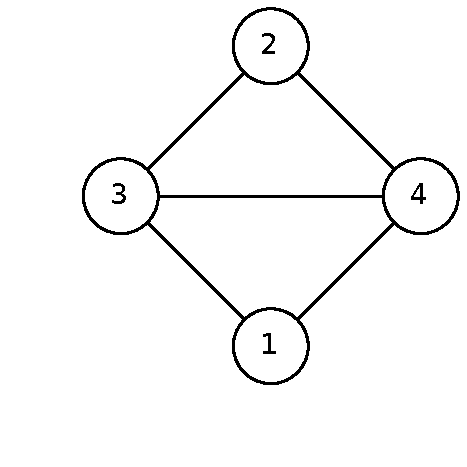
\includegraphics[width=0.8\linewidth]{dots/grafo1}

		\end{figure}
		\end{column}
		\begin{column}{0.65\textwidth}
			\begin{itemize}
				\item $V = \{1, 2, 3, 4\}$
				\item $E = \{\{1, 3\}, \{1, 4\}, \{2, 3\}, \{2, 4\}, \{3, 4\}\}$
				\item $n = 4$ e $m = 5$
			\end{itemize}
		\end{column}
	\end{columns}
\end{frame}



\begin{frame}{Definições básicas}
	\framesubtitle{Grafos dirigidos}
	
	\begin{itemize}
		\item Grafos podem conter direção nas suas arestas.
		\item Neste caso, chamamos de \textbf{grafo dirigido} ou \textbf{grafo direcionado}.
		\item Abreviamos como digrafo (do inglês \textit{digraph} -- \textit{directed graph}).
		\item Cada aresta $e \in E$ é um par direcionado $e = (u, v)$.
		\begin{itemize}
			\item $e = (u, v) \ne e' = (v, u)$.
			\item \textbf{Convenção:} \textit{arestas} são não-direcionadas e \textit{arcos} são direcionados.
		\end{itemize}
	
		\pause
		\item {\color{magenta}Representação visual:}
	\end{itemize}

	\vspace{-12pt}
	
	\begin{columns}
		\begin{column}{0.35\textwidth}
			\begin{figure}		
				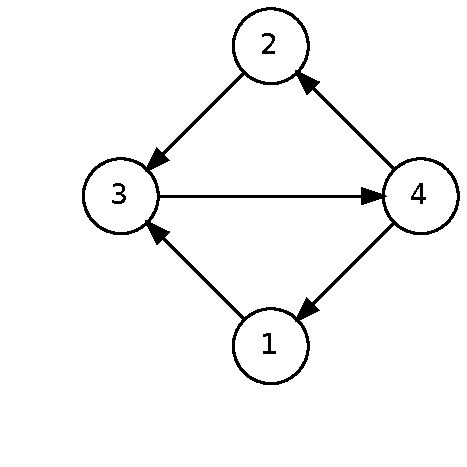
\includegraphics[width=0.8\linewidth]{dots/grafo2}

			\end{figure}
		\end{column}
		\begin{column}{0.65\textwidth}
			\begin{itemize}
				\item $V = \{1, 2, 3, 4\}$
				\item $E = \{(1, 3), (2, 3), (3, 4), (4, 1), (4, 2)\}$
				\item $n = 4$ e $m = 5$
			\end{itemize}
		\end{column}
	\end{columns}
\end{frame}



\begin{frame}{Definições básicas}
	\framesubtitle{Exemplo -- Rede social de \textit{Game of Thrones}}

	\begin{figure}
		\centering
		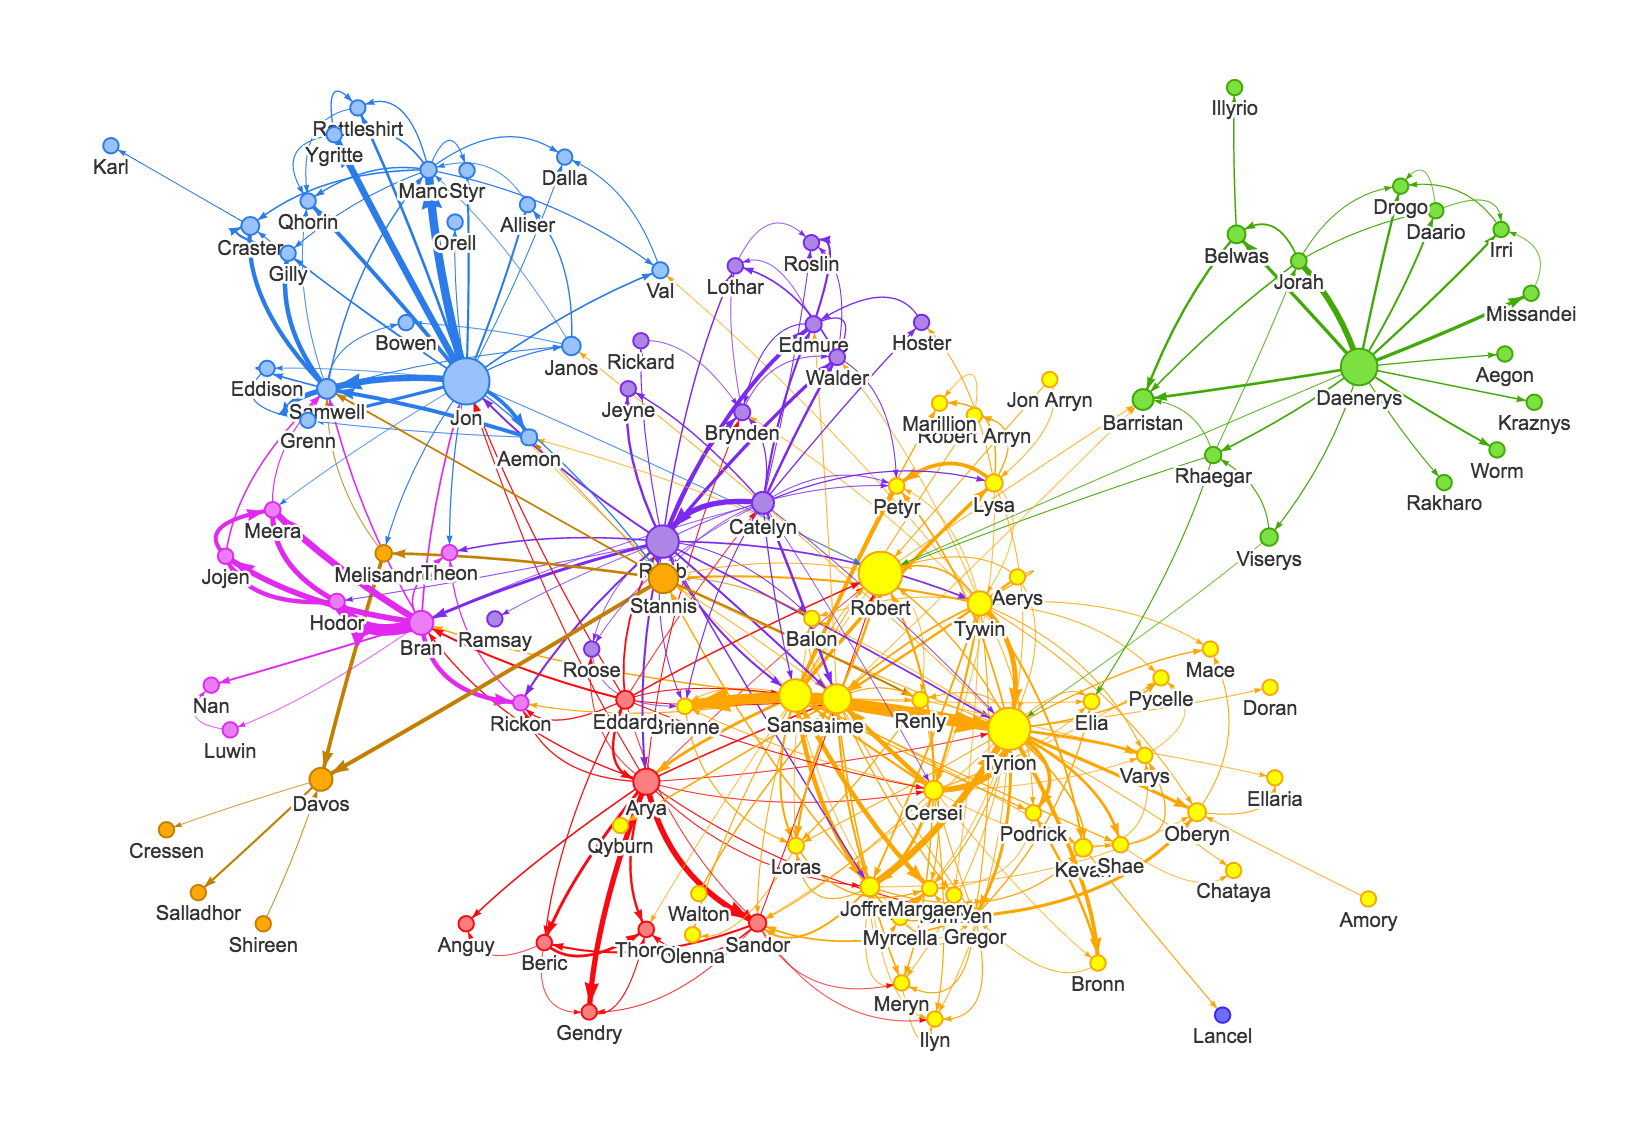
\includegraphics[width=0.9\linewidth]{img/graph-of-thrones}
	\end{figure}
\end{frame}



\begin{frame}{Definições básicas}
	\framesubtitle{Outros exemplos}

	\begin{table}
		\centering
		\begin{tabular}{lll}
			\hline
			\textbf{Grafo} & \textbf{Nodos} & \textbf{Arestas} \\
			\hline
			Comunicação & computador & cabo de fibra ótica \\
			Circuito eletrônico & componentes & fio \\
			Transporte & interceção de ruas & vias \\
			Linhas aéreas & aeroportos & rotas aéreas \\
			Jogo & posições em um tabuleiro & movimentos possíveis \\
			Internet & páginas & links \\
			Dependências & cursos & pré-requisitos \\
			\hline
		\end{tabular}
	\end{table}
\end{frame}



\begin{frame}[t]{Representação de grafos}
	\framesubtitle{Matriz de adjacências}
	
	\begin{itemize}
		\item {\color{magenta}Matriz $n \times n$ em que $A_{uv} = 1$ se $(u, v)$ é uma aresta.}
		\item Complexidade de espaço: $\Theta(n^2)$.
		\item Checar se $(u, v)$ é uma aresta: $\Theta(1)$.
		\item Recuperar todos os vizinhos de um vértice $v$: $\Theta(n)$.
		\item Recuperar todas as arestas: $\Theta(n^2)$.
	\end{itemize}
	
	\pause
	
	\begin{columns}[c]
		\begin{column}{0.18\textwidth}\end{column}
		\begin{column}{0.6\textwidth}

			\begin{columns}[c]		
				\only<2>{
				\begin{column}{3.5cm}
					\begin{figure}
						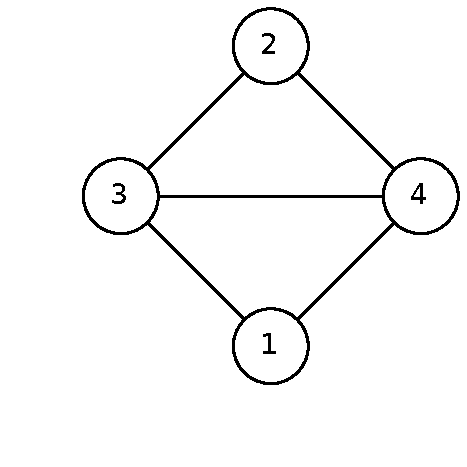
\includegraphics[width=1\linewidth]{dots/grafo3}

					\end{figure}
				\end{column}
				
				\begin{column}{3.5cm}
					\begin{table}
						\def\arraystretch{1.2}
						\color{black}
						\begin{tabular}{c|cccc}
							& \textbf{1} & \textbf{2} & \textbf{3} & \textbf{4} \\ \hline
							\textbf{1} &     0      &     0      &     1      &     1      \\
							\textbf{2} &     0      &     0      &     1      &     1      \\
							\textbf{3} &     1      &     1      &     0      &     1      \\
							\textbf{4} &     1      &     1      &     1      &     0
						\end{tabular}
					\end{table}
				\end{column}
				}
			
				\only<3>{
				\begin{column}{3.5cm}
					\begin{figure}
						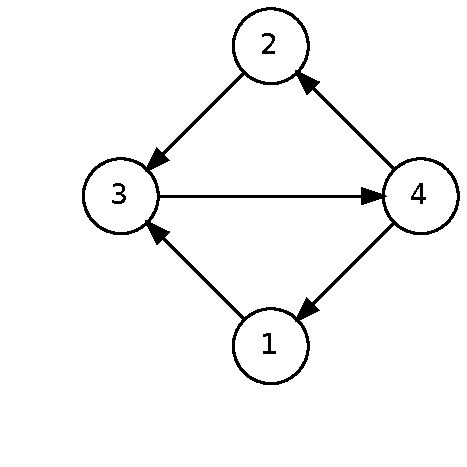
\includegraphics[width=1\linewidth]{dots/grafo4}

					\end{figure}
				\end{column}
				
				\begin{column}{3.5cm}
					\begin{table}
						\def\arraystretch{1.2}
						\color{black}
						\begin{tabular}{c|cccc}
							& \textbf{1} & \textbf{2} & \textbf{3} & \textbf{4} \\ \hline
							\textbf{1} &     0      &     0      &     1      &     0      \\
							\textbf{2} &     0      &     0      &     1      &     0      \\
							\textbf{3} &     0      &     0      &     0      &     1      \\
							\textbf{4} &     1      &     1      &     0      &     0
						\end{tabular}
					\end{table}
				\end{column}
				}
		\end{columns}	
		
		\end{column}
		\begin{column}{0.18\textwidth}\end{column}
	\end{columns}
\end{frame}



\begin{frame}[t]{Representação de grafos}
	\framesubtitle{Listas de adjacências}
	
	\vspace{-5pt}
	
	\begin{itemize}
		\item {\color{magenta}Vetor indexado pelos nodos com listas de vizinhos.}
		\item Complexidade de espaço: $\Theta(m + n)$.
		\item Checar se $(u, v)$ é uma aresta: $\Theta(grau(u))$.
		\item Recuperar todos os vizinhos de um vértice $v$: $\Theta(grau(v))$.
		\begin{itemize}
			\item O grau de um vértice é o número de vizinhos que ele possui.
		\end{itemize}
		\item Recuperar todas as arestas: $\Theta(m + n)$.
	\end{itemize}

	\pause
	
	\only<2>{
		\begin{tikzpicture}[remember picture,overlay,shift={(current page.center)}]
			\node [text width=3.5cm] at (-3, -2.3) {%
				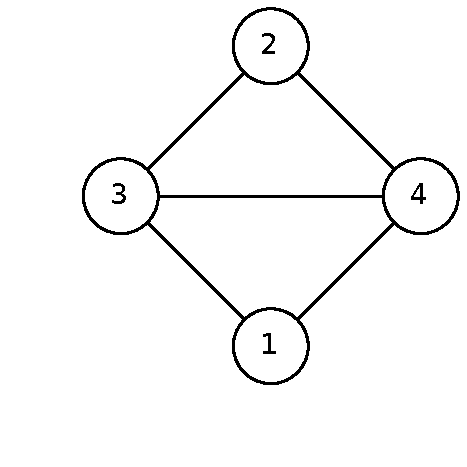
\includegraphics[width=1\linewidth]{dots/grafo3}
%
			};
		
			\node [text width=5.5cm] at (2, -2.3) {%
				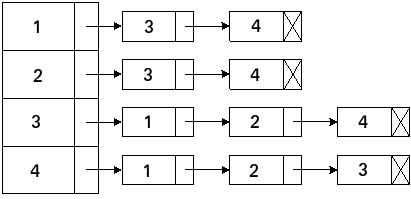
\includegraphics[width=\linewidth]{img/adjacency-list}
			};
		\end{tikzpicture}
	}

	\only<3>{
		\begin{tikzpicture}[remember picture,overlay,shift={(current page.center)}]
		\node [text width=3.5cm] at (-3, -2.3) {%
			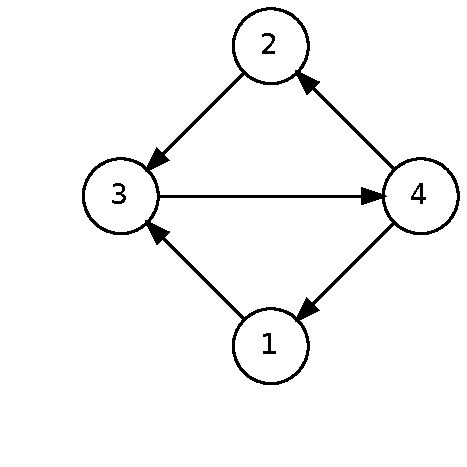
\includegraphics[width=1\linewidth]{dots/grafo4}
%
		};
		
		\node [text width=4.2cm] at (1.4, -2.3) {%
			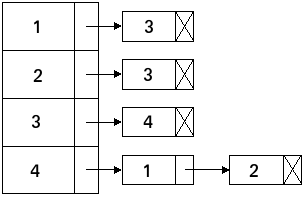
\includegraphics[width=\linewidth]{img/adjacency-list-2}
		};
		\end{tikzpicture}
	}
\end{frame}



\begin{frame}{Representação de grafos}
	\framesubtitle{Implementação}

	\begin{itemize}
		\item A lista de adjacências é uma melhor representação para grafos.
		\item Qual estrutura básica utilizar? \textbf{Vetores} ou \textbf{listas encadeadas}?
		
		\item {\color{magenta}Vetores:} são ideais para implementação de grafos.
		\begin{itemize}
			\item Permitem o acesso aleatório à estrutura.
			\item Não demandam tempo adicional para caminhamento na estrutura.
		\end{itemize}
	
		\item {\color{magenta}Listas:} são ideais para estruturas dinâmicas.
		\begin{itemize}
			\item Permitem a inserção e remoção de elementos em tempo constante.
			\item Não demandam tempo adicional para modificações na estrutura.
		\end{itemize}
	
		\item {\color{magenta}Dica geral:}
		\begin{itemize}
			\item Para grafos estáticos ou com pouca variação: \textbf{vetores}.
			\item Para grafos dinâmicos e com muita variação: \textbf{encadeamento}.
		\end{itemize}
	\end{itemize}
\end{frame}



\begin{frame}{Exercício}
	\framesubtitle{Implementação de grafos}
	
	\begin{enumerate}
		\item Implemente uma classe grafo para modelar essa estrutura de dados. Utilize a representação por listas de adjacências e implemente versões utilizando vetores e listas encadeadas. Utilize as classes criadas para armazenar grafos de um domínio específico à sua escolha. Implemente rotinas para calcular o grau de um vértice, sua lista de vizinhos e o tamanho do grafo.
	\end{enumerate}
\end{frame}



\begin{frame}{Caminhos e conectividade de grafos}
	
	\begin{itemize}
		\item Um \textbf{\color{magenta}caminho} em um grafo não direcionado $G = (V, E)$ é uma sequência de vértices $v_1, v_2, \dots, v_k$, onde cada par consecutivo $v_{i-1}, v_i$ está ligado por uma aresta em $E$.
		\begin{itemize}
			\item O mesmo conceito se aplica a grafos direcionados (caminho direcionado).
		\end{itemize}
		
		\item Um caminho é \textbf{simples} se todos os seus vértices são diferentes.
		
		\pause
		\item Um grafo é \textbf{\color{magenta}conectado} (ou conexo) se para todo par de vértices $u$ e $v$, existe um caminho conectando $u$ a $v$.
		\begin{itemize}
			\item Um grafo direcionado é \textbf{fortemente conectado} se para todo par de vértices $u$ e $v$, existe caminhos conectando $u$ a $v$ e $v$ a $u$.
		\end{itemize}
	\end{itemize}

	\pause
	\begin{figure}
		\centering
		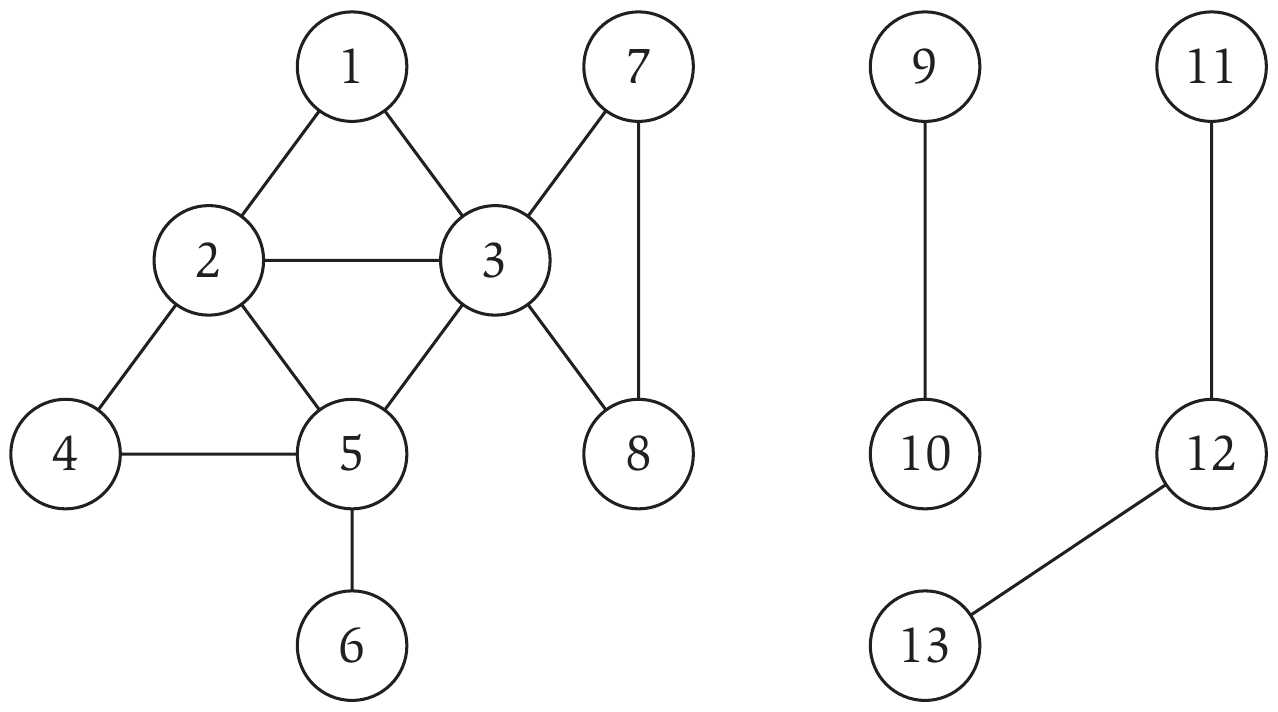
\includegraphics[width=0.55\linewidth]{img/conectividade}
	\end{figure}
\end{frame}



\begin{frame}{Ciclos em grafos}
	
	\begin{itemize}
		\item Um \textbf{\color{magenta}ciclo} é um caminho $v_1, v_2, \dots, v_k$, em que $v_1 = v_k$, $k > 2$ e todos os $k - 1$ primeiros vértices são distintos.
		\begin{itemize}
			\item O caminho $1, 2, 4, 5, 3, 1$ é um ciclo no grafo abaixo.
			\item O caminho $3, 7, 8, 3$ é um ciclo no grafo abaixo.
		\end{itemize}
	\end{itemize}

	\begin{figure}
		\centering
		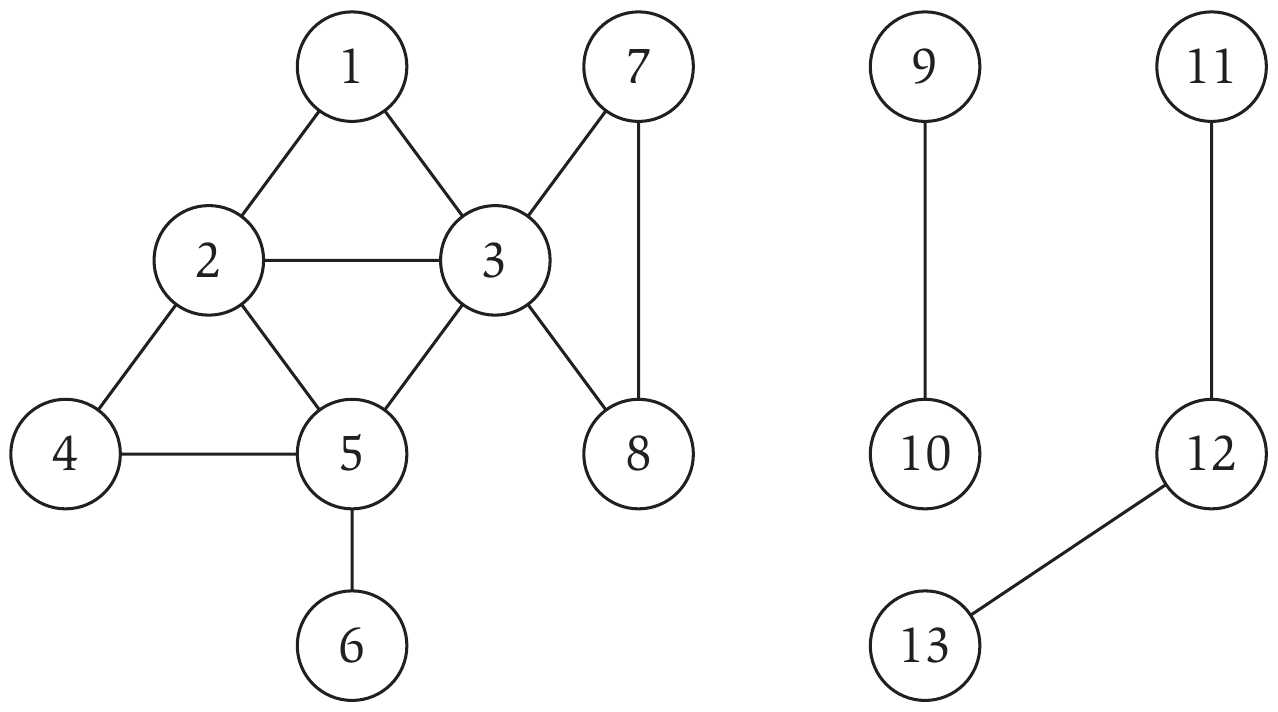
\includegraphics[width=0.375\linewidth,trim={0 0 15cm 0},clip]{img/conectividade}
	\end{figure}
\end{frame}



\begin{frame}{Árvores}

	\begin{itemize}
		\item Um grafo é uma \textbf{\color{magenta}árvore} se ele é conectado e não contém ciclos.
		\begin{itemize}
			\item Ou seja, uma árvore é um grafo conectado sem ciclos.
		\end{itemize}
		\item Qualquer vértice pode ser escolhido como raiz da árvore para uma organização gráfica comum de árvores.
	\end{itemize}

	\begin{figure}
		\centering
		
\includegraphics[width=0.85\linewidth]{img/arvores}
	\end{figure}
\end{frame}



\begin{frame}{Árvores}

	\begin{itemize}
		\item {\color{magenta}Teorema:} seja $G$ um grafo não-direcionado com $n$ vértices. Quaisquer duas afirmações verdadeiras implica na terceira.
		\begin{enumerate}
			\item $G$ é conectado.
			\item $G$ não contém ciclos.
			\item $G$ possui $n - 1$ arestas.
		\end{enumerate}
	\end{itemize}
	
	\begin{figure}
		\centering
		
\includegraphics[width=0.85\linewidth]{img/arvores}
	\end{figure}
\end{frame}



\begin{frame}{Buscas -- percorrendo um grafo}

	\begin{itemize}
		\item {\color{magenta}Busca:} visitação sistemática dos vértices do grafo.
		\begin{itemize}
			\item Buscar um vértice determinado.
			\item Procedimento para resolução de outros problemas relacionados.
		\end{itemize}
	
		\item Estratégias básicas (ordem de visitação):
		\begin{itemize}
			\item Busca em largura (\textit{breadth-first search} -- BFS).
			\item Busca em profundidade (\textit{depth-first search} -- DFS).
		\end{itemize}
	
		\item Dado um vértice inicial, explora o grafo.
	\end{itemize}

	\begin{figure}
		\centering
		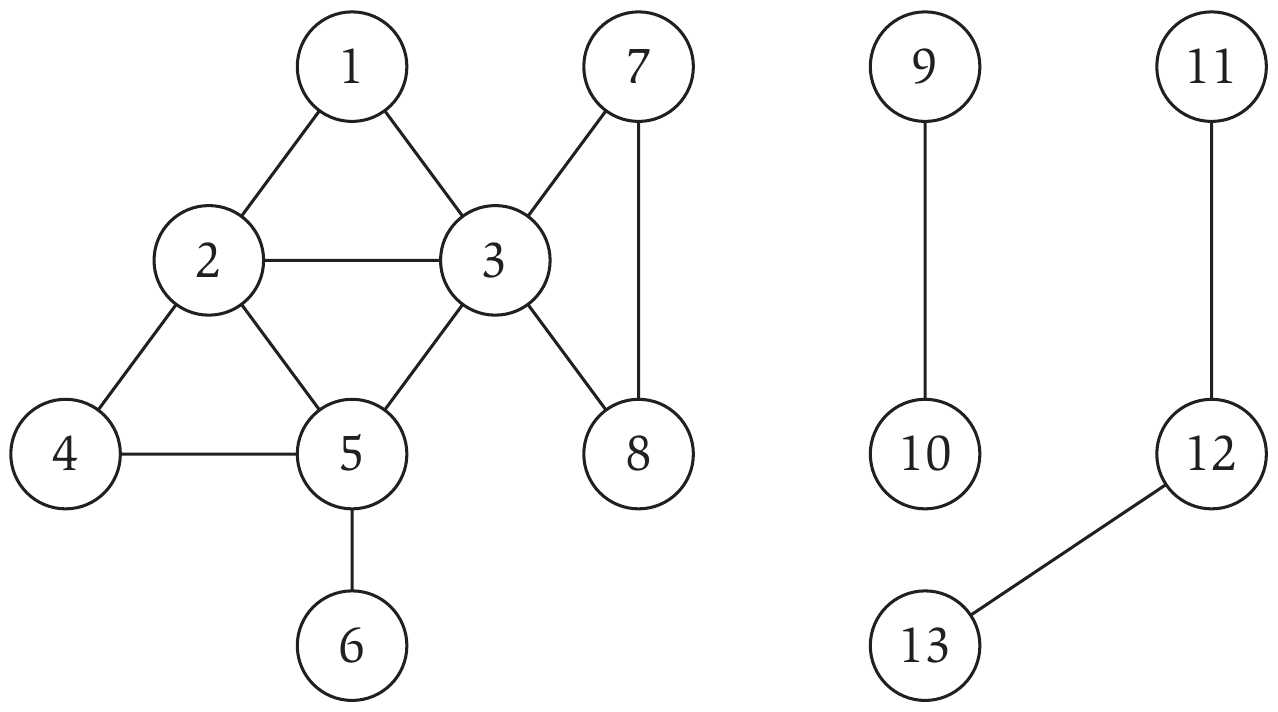
\includegraphics[width=0.375\linewidth,trim={0 0 15cm 0},clip]{img/conectividade}
	\end{figure}
\end{frame}



\begin{frame}{Busca em largura}
	\framesubtitle{Estratégia}
	
	\begin{itemize}
		\item Na \textbf{\color{magenta}busca em largura}, o grafo é explorado por camadas a partir do vértice de início.
		
		\begin{enumerate}
			\item Visita o vértice atual.
			\item Inclui seus vizinhos ainda não visitados e na lista para exploração.
			\item Seleciona o vértice de menor camada e vai para o passo 1.
		\end{enumerate}
	
		\medskip
		\item Seja $L_i$ o conjunto de vértices da camada $i$.
		\item Estes vértices estão a uma distância mínima de $i$ do vértice de início.
		\item Todo vértice em $L_{i-1}$ é visitado antes dos vértices em $L_i$.
		\item Só existe um caminho de $u$ a $v$ se e somente se $v$ estiver em uma das camadas da busca a partir de $u$ (e vice-versa).
	\end{itemize}
\end{frame}



\begin{frame}{Busca em largura}
	\framesubtitle{Funcionamento}

	\begin{itemize}
		\item Seja o grafo abaixo.
	\end{itemize}
	
	\vspace{-8pt}
	
	\begin{figure}
		\centering
		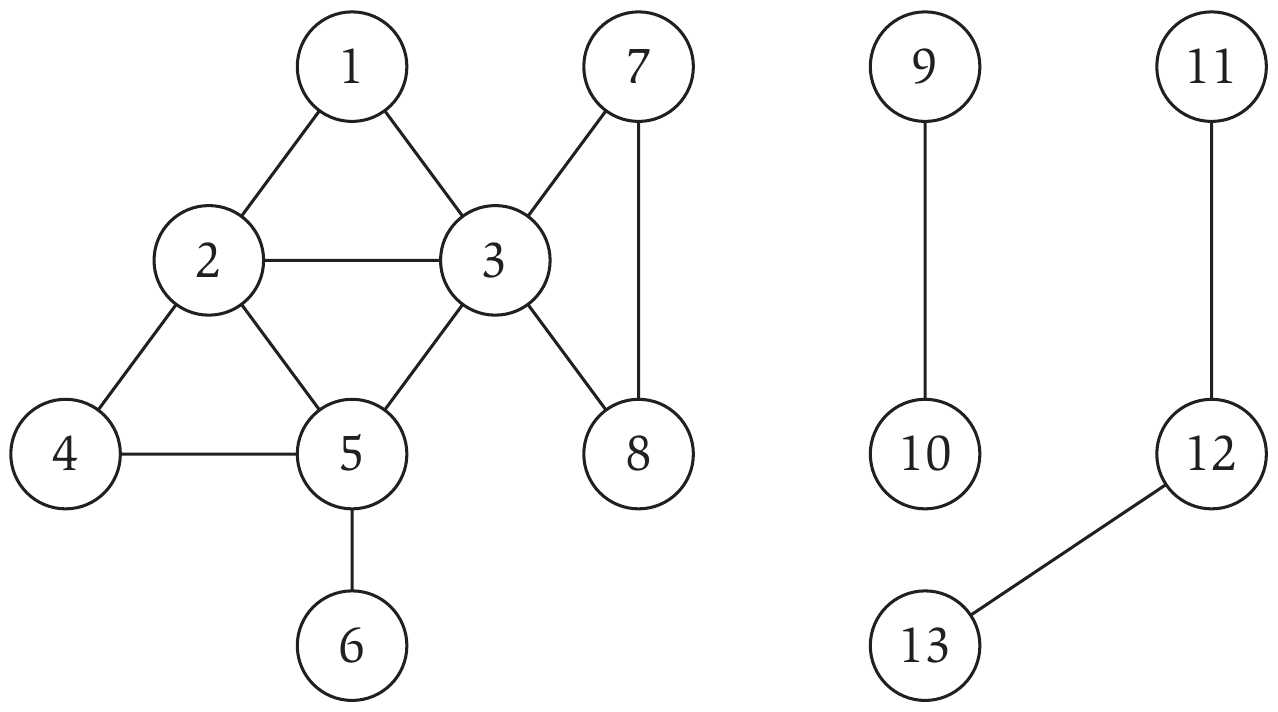
\includegraphics[width=0.25\linewidth,trim={0 0 15cm 0},clip]{img/conectividade}
	\end{figure}
	
	\vspace{-8pt}
	
	\begin{itemize}
		\item Execução da busca em largura (camadas de visitação):
	\end{itemize}
	
	\vspace{-2pt}
	
	\begin{figure}
		\centering
		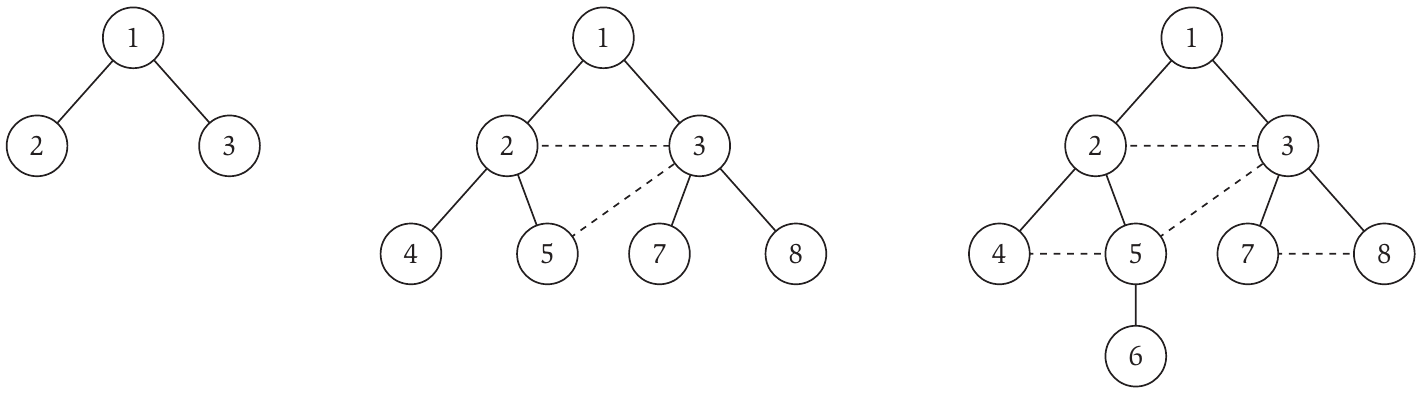
\includegraphics[width=0.9\linewidth,trim={0 0 0 0},clip]{img/busca-largura}
	\end{figure}
\end{frame}



%\begin{frame}{Busca em largura}
%	\framesubtitle{Complexidade}
%
%	\begin{itemize}
%		\item {\color{magenta}Teorema:} a busca em largura executa em tempo $O(n + m)$.
%		
%		\bigskip
%		
%		\item {\color{magenta}Prova}
%		
%		\begin{itemize}
%			\item Complexidade $O(n^2)$:
%			\begin{itemize}
%				\item Existem no máximo $n^2$ listas $L[i]$.
%			\end{itemize}
%		\end{itemize}
%		
%	\end{itemize}
%
%\end{frame}



\begin{frame}{Busca em profundidade}
	\framesubtitle{Estratégia}
	
	\begin{itemize}
		\item Na \textbf{\color{magenta}busca em profundidade}, o grafo é explorado indo o mais profundo possível nas camadas, antes de explorar vértices da mesma camada.
		
		\begin{enumerate}
			\item Visita o vértice atual.
			\item Inclui seus vizinhos ainda não visitados e na lista para exploração.
			\item Seleciona o vértice de \textbf{maior} camada e vai para o passo 1.
		\end{enumerate}
		
		\medskip
		\item O algoritmo caminha para mais longe na busca, antes de visitar vizinhos mais próximos.
		\item Só existe um caminho de $u$ a $v$ se e somente se $v$ estiver em uma das camadas da busca a partir de $u$ (e vice-versa).
	\end{itemize}
\end{frame}



\begin{frame}{Busca em profundidade}
	\framesubtitle{Funcionamento}

	\begin{itemize}
		\item Seja o grafo abaixo.
	\end{itemize}
	
	\vspace{-9pt}
	
	\begin{figure}
		\centering
		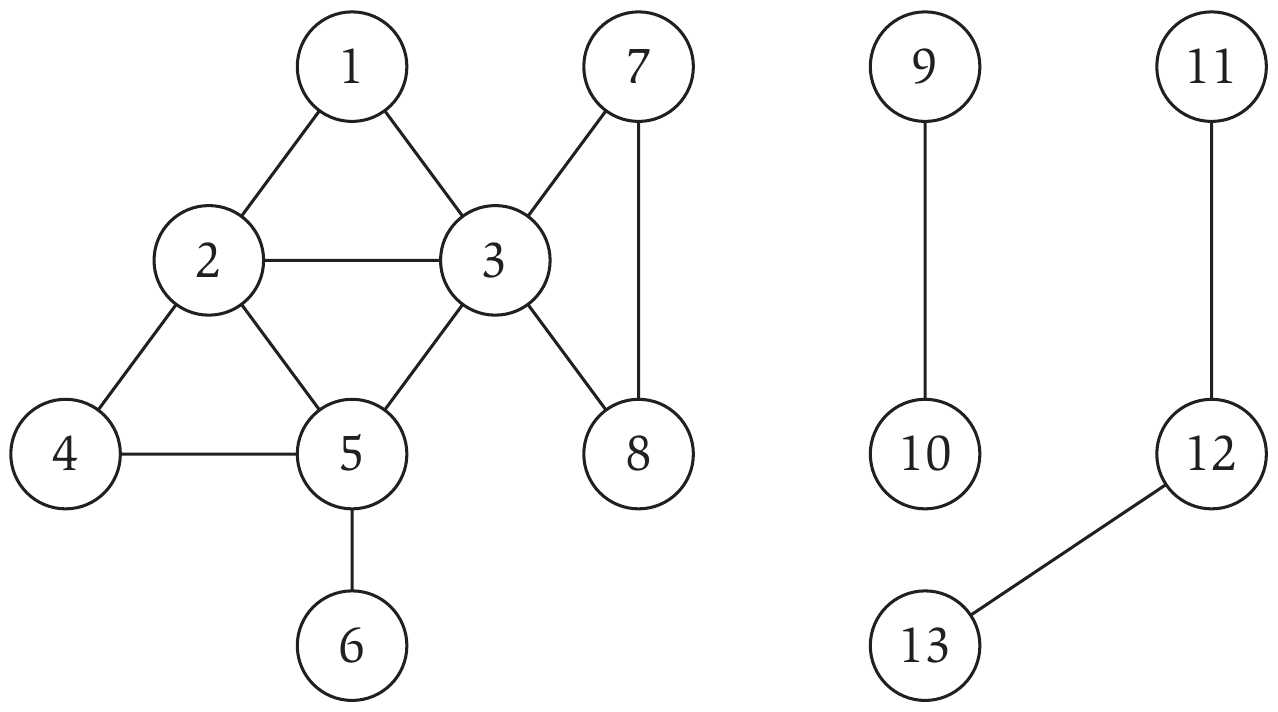
\includegraphics[width=0.2\linewidth,trim={0 0 15cm 0},clip]{img/conectividade}
	\end{figure}
	
	\vspace{-8pt}
	
	\begin{itemize}
		\item Execução da busca em profundidade (ordem de visitação):
	\end{itemize}
	
	\vspace{-4pt}
	
	\begin{figure}
		\centering
		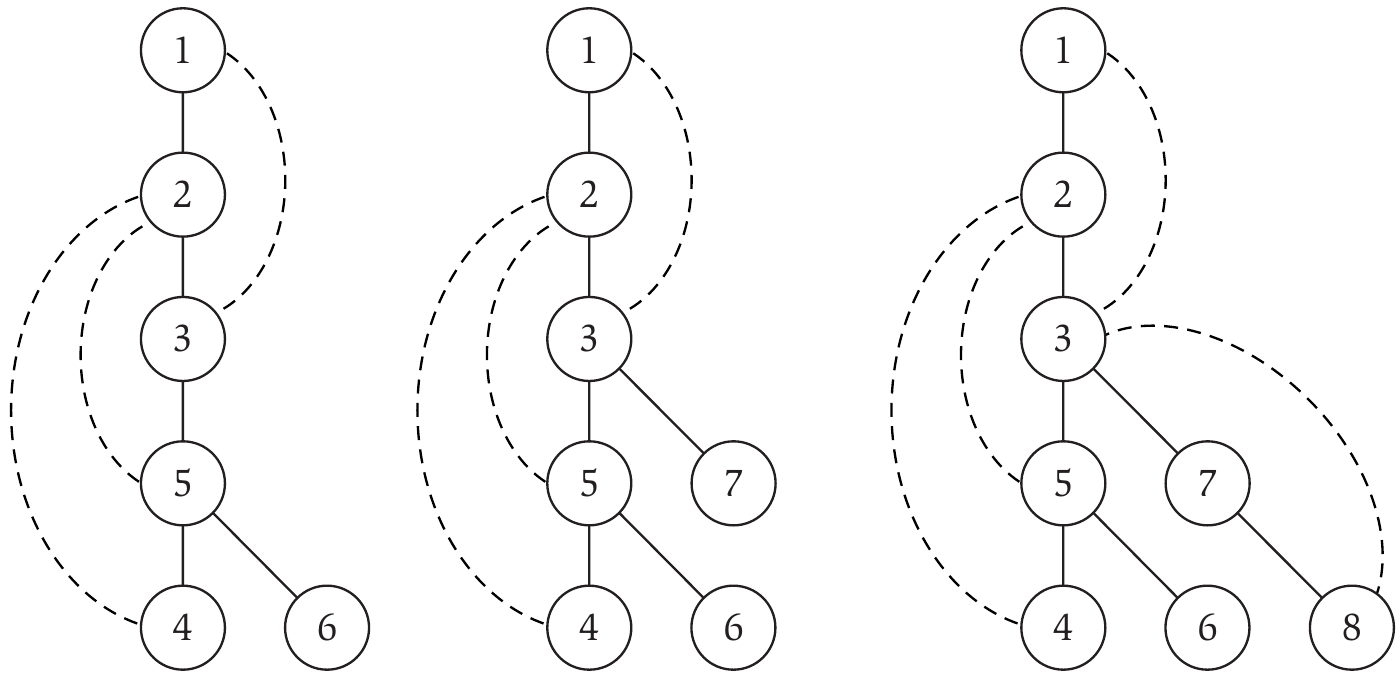
\includegraphics[width=0.65\linewidth,trim={0 0 0 0},clip]{img/busca-profundidade}
	\end{figure}
\end{frame}



\begin{frame}[t]{Estratégia básica de busca}
	\framesubtitle{Detalhes de implementação}
	
	\begin{algorithm}[H]
		\DontPrintSemicolon
		
		$A \gets \{s\}$\;
		
		\While{$A \neq \emptyset$}{
			$v \gets$ extract vertex from $A$\;
			Visit vertex $v$\;
			Let $N(v)$ the set of unvisited neighbors of $v$\;
			$A \gets A \cup N(v)$\;
		}
		
		\caption{\texttt{search(Vertex s)}}
	\end{algorithm}
	
	\medskip
	
	\only<2>{
	\begin{itemize}
		
		\item Estruturas de dados básicas:
		\begin{itemize}
			\item Para implementar a busca em largura, $A$ é uma \textbf{fila}.
			\item Para implementar uma busca em profundidade, $A$ é uma \textbf{pilha}.
			\item Para outras estratégias, $A$ pode ser uma \textbf{fila de prioridades}.
		\end{itemize}
	\end{itemize}
	}
	
	
	\only<3>{
	\begin{itemize}
		\item Complexidade:
		\begin{itemize}
			\item A recuperação de vizinhos não visitados está limitada ao grau do nodo.
			\item O somatório dos graus de cada nodo é $2m$.
			\item Logo, a complexidade do laço é $O(m)$.
			\item É necessário um esforço inicial, para criar um vetor \texttt{discovered} para armazenar a visitação de cada vértice, demandando $O(n)$.
			\item Logo, as buscas estudadas executam em tempo $O(m + n)$.
		\end{itemize}
	\end{itemize}
	}	
\end{frame}



\begin{frame}{Buscas em grafos}
	\framesubtitle{Aplicações}
	
	\begin{itemize}
		\item Encontrar um caminho entre um par de vértices.
		\item Detectar ciclos em um grafo.
		\item Resolver jogos de quebra-cabeça.
		\item Descobrir links entre páginas em um buscador.
		\item Encontrar amigos próximos em uma rede social.
		\item Broadcast em redes.
	\end{itemize}
\end{frame}



\begin{frame}{Exercício}
	\framesubtitle{Buscas em grafos}
	
	\begin{enumerate}
		\item Implemente os algoritmos de busca em largura e profundidade para o grafo criado no exercício anterior. Considere que o grafo é conectado e utilize o algoritmo para as seguintes tarefas:
		\begin{enumerate}
			\item Encontrar um determinado vértice no grafo.
			\item Retornar o menor caminho entre um par de vértices.
			\item Imprimir toda a estrutura do grafo.
		\end{enumerate}
	\end{enumerate}
\end{frame}



\begin{frame}{Componente conexo}
	
	\begin{itemize}
		\item Dizemos que $C$ é o \textbf{\color{magenta}componente conexo} de um vértice $s$, se e somente se, todos os vértices alcançáveis a partir de $s$ estão em $C$.
		\item Ou seja, é o conjunto de vértices que estão conectados a $s$.
		\item Exemplos: 
		\begin{itemize}
			\item O componente conexo de $12$ é $\{11, 12, 13\}$.
			\item O componente conexo de $5$ é $\{1, 2, 3, 4, 5, 6, 7, 8\}$.
		\end{itemize}
		
	\end{itemize}

	\begin{figure}
		\centering
		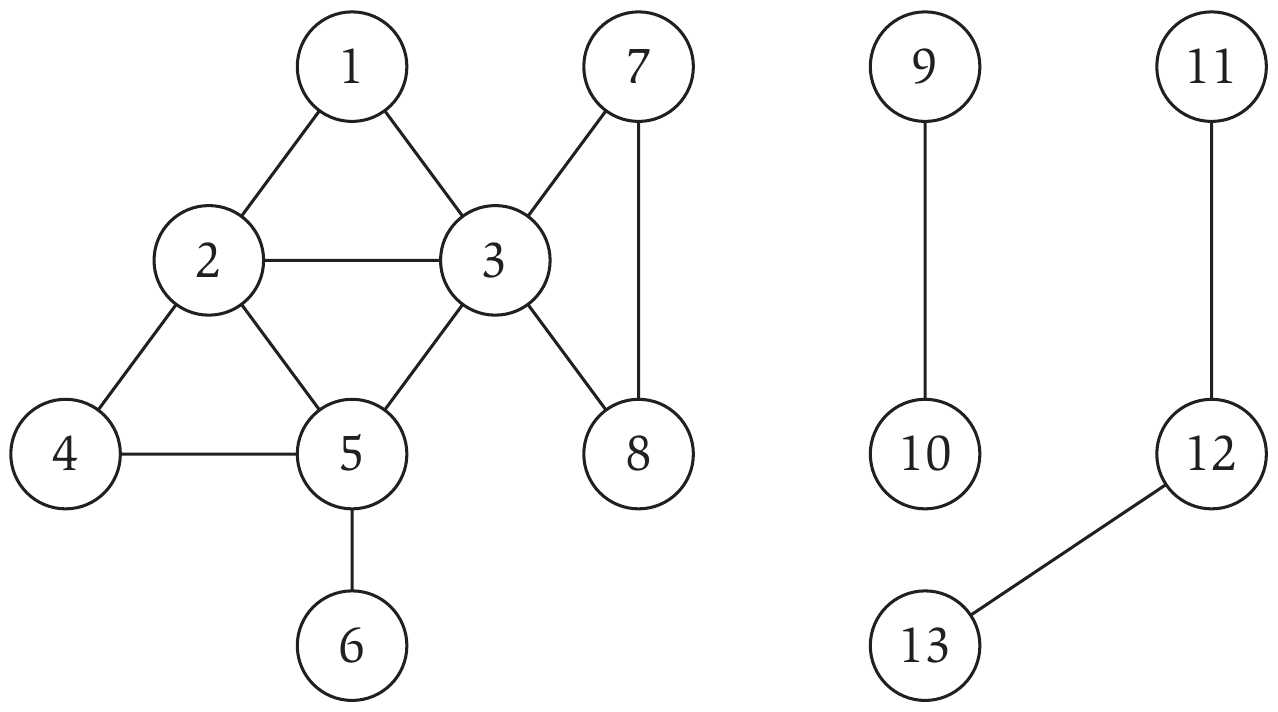
\includegraphics[width=0.55\linewidth]{img/conectividade}
	\end{figure}
\end{frame}



\begin{frame}{Componente conexo}
	\framesubtitle{Aplicações}
	
	\begin{itemize}
		\item {\color{magenta}Flood fill:} um desenho é representado por um grafo de píxels. Ao clicar em um píxel para pintura, toda a área da mesma cor é pintada. Ou seja, todo o componente conexo de uma determinada cor.
	\end{itemize}
	
	\begin{figure}
		\centering
		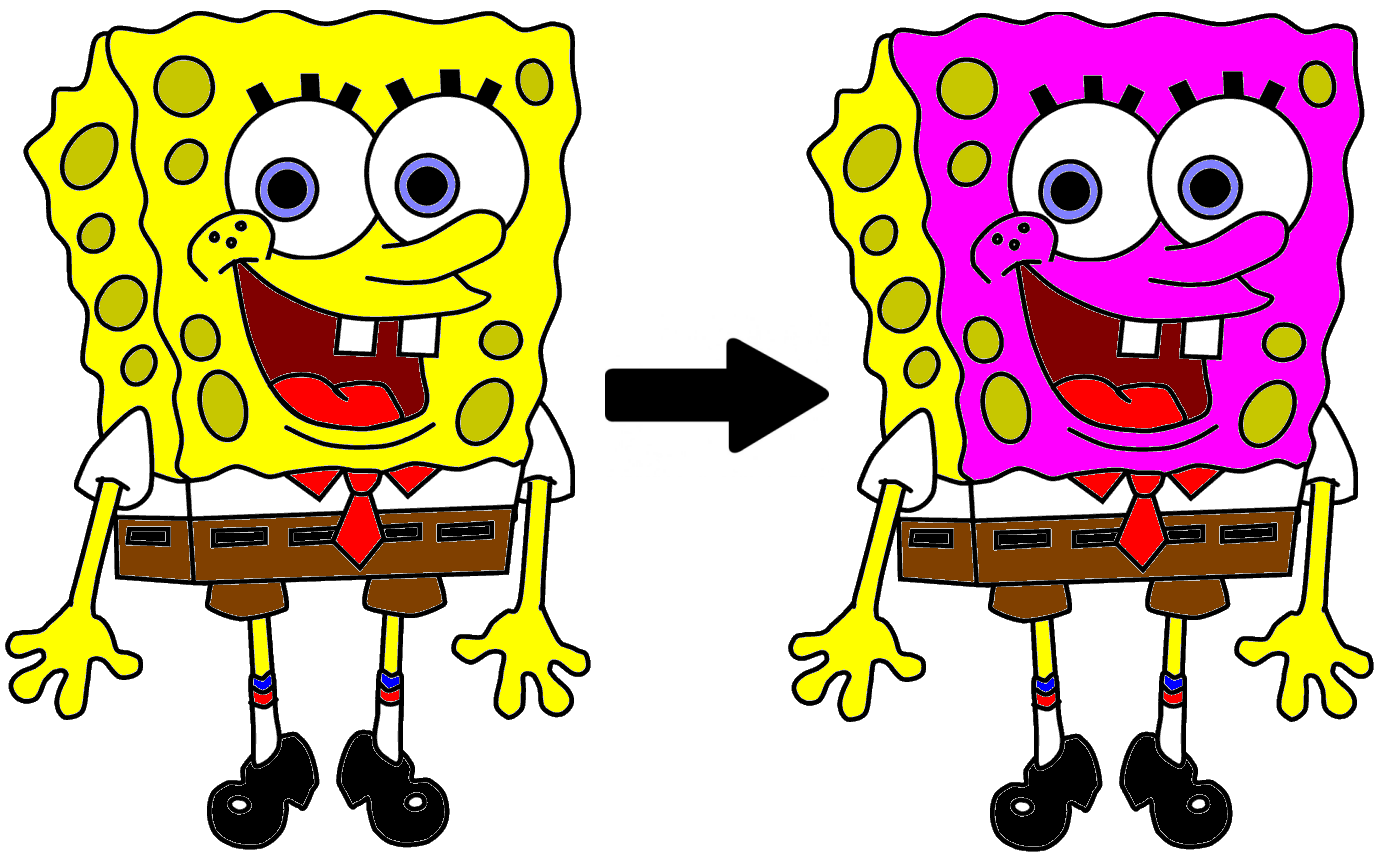
\includegraphics[width=0.55\linewidth]{img/flood-fill}
	\end{figure}
\end{frame}



\begin{frame}{Componente conexo}
	\framesubtitle{Algoritmo}
	
	\begin{algorithm}[H]
		\DontPrintSemicolon
		
		Let $C$ be the set of nodes to which $s$ has a path\;
		$C \gets \{s\}$\;
		
		\While{there is an edge $(u, v)$ where $u \in C$ and $v \notin C$}{
			Add $v$ to $C$\;
		}
		
		\caption{\texttt{connected-component(Vertex s)}}
	\end{algorithm}

	\begin{itemize}
		\item Uma boa estratégia é utilizar as buscas estudadas para obter o componente conexo de um vértice inicial.
		\begin{itemize}
			\item Busca largura/profundidade definirão a ordem de inserção dos vértices. 
		\end{itemize}
	
		\item {\color{magenta}Propriedade:} se um nodo $v$ está conectado a $s$, ele estará no conjunto $C$ produzido pelo algoritmo.
		\begin{itemize}
			\item As buscas exploram todos os vértices alcançáveis a partir do vértice inicial.
		\end{itemize}
	\end{itemize}
\end{frame}



\begin{frame}{Encontrando todos os componentes conexos}
	
	\begin{itemize}
		\item Executar a busca (largura, por exemplo) repetidamente:
		\begin{enumerate}
			\item Executa a busca a partir do vértice $s$, obtendo seu componente conexo.
			\item Repete o passo anterior, iniciando por um vértice não marcado.
		\end{enumerate}
		\item Ao final, o algoritmo descobre todos os componentes conexos.
		
		\pause
		\medskip
		\item \textbf{Complexidade:}
		\begin{itemize}
			\item O algoritmo de busca executa em tempo $O(m + n)$.
			\item Porém, ele se limita ao componente conexo em questão.
			\item Na soma de todos os componentes conexos, o algoritmo demanda tempo total de $O(m + n)$.
		\end{itemize}
	
		\pause
		\medskip
		\item Como podemos adaptar esse algoritmo para obter o maior componente conexo?
	\end{itemize}
\end{frame}



\begin{frame}{Exercício}
	\framesubtitle{Componente conexo}
	
	\begin{enumerate}
		\item Crie um grafo para modelar a rede interna de telefonia de uma empresa. Os departamentos da empresa são os vértices e as arestas são as conexões cabeadas existentes na rede de telefonia. Neste sentido, os departamentos da empresa possuem ligações entre si. Esse grafo deve ser desconectado, representando grupos de departamentos que estão isolados na rede interna. Dado um grafo dessa natureza, crie um algoritmo que receba um departamento e retorne seu componente conexo. Crie também um algoritmo para determinar o maior componente conexo da empresa.
	\end{enumerate}
\end{frame}



\begin{frame}{Operações em grafos dirigidos}
	\framesubtitle{Buscas}
	
	\begin{itemize}
		\item Em \textbf{grafos não-dirigidos} uma busca é capaz de encontrar o componente conexo a partir de um vértice $s$.
		\item Em \textbf{grafos dirigidos} uma busca encontra apenas o conjunto de vértices para os quais $s$ tem um caminho.
		\item Exemplos:
	\end{itemize}
	
	\vspace{-10pt}
	
	\begin{figure}
		\begin{tikzpicture}[
			> = stealth,
			shorten > = 1pt,
			auto,
			node distance = 3cm,
			semithick,
			scale=0.5,
			transform shape
		]
		
			\tikzset{every state}=[
				draw = black,
				thick,
				fill = white,
				minimum size = 1mm
			]
			
			\node[state, fill=blue!40] (y1) {$C$};
			\node[state, fill=blue!40] (y2) [right=of y1] {$D$};
			\node[state, fill=blue!40] (x1) [above=of y1]{$A$};
			\node[state, fill=blue!40] (x2) [above=of y2] {$B$};
			
			\path[-] (x1) edge  node[] {} (y1);
			\path[-] (y1) edge  node[pos=0.25,below right] {} (x2);
			\path[-] (x1) edge  node[pos=0.25,above right] {} (y2);
			\path[-] (x2) edge  node[] {} (y2);
			\path[-] (x2) edge  node[above] {} (x1);
			\path[-] (y2) edge  node[above] {} (y1);
		
			\node[state, fill=blue!40] (A) [right=of x2]{$A$};
			\node[state, fill=blue!40] (B) [right=of A] {$B$};
			\node[state, fill=blue!40] (C) [right=of y2]{$C$};
			\node[state] (D) [right=of C] {$D$};
			
			\path[->] (A) edge  node[] {} (C);
			\path[->] (C) edge  node[pos=0.25,below right] {} (B);
			\path[->] (D) edge  node[pos=0.25,above right] {} (A);
			\path[->] (D) edge  node[] {} (B);
			\path[->] (B) edge  node[above] {} (A);
			\path[->] (D) edge  node[above] {} (C);
			
		\end{tikzpicture}
	\end{figure}

	\begin{itemize}
		\item No primeiro grafo, todos os vértices são visitados pela busca a partir de $A$. No segundo grafo, apenas aqueles com caminho desde $A$.
	\end{itemize}
\end{frame}



\begin{frame}{Operações em grafos dirigidos}
	\framesubtitle{Conexidade}
	
	\begin{itemize}
		\item Em \textbf{grafos não-dirigidos}, o grafo é conexo se entre todo par de vértices existe um caminho.
		
		\item Em \textbf{grafos dirigidos}:
		\begin{itemize}
			\item {\color{magenta}Fracamente conexo:} entre todo par de vértices existe uma ligação.
			\begin{itemize}
				\item Dica: ignorando as direções dos arcos, verifica se o grafo não-direcionado subjacente é conexo.
			\end{itemize}
			
			\item {\color{magenta}Fortemente conexo:} entre todo par de vértices $\{u, v\}$ existe um caminho de $u$ para $v$ e um caminho de $v$ para $u$.
			\begin{itemize}
				\item Ou seja, os vértices tem que ser mutuamente alcançáveis.
			\end{itemize}
		\end{itemize}
	
		\item Exemplos -- (1) fracamente conexo e (2) fortemente conexo:
	\end{itemize}

	\begin{figure}
		\begin{tikzpicture}[
		> = stealth,
			shorten > = 1pt,
			auto,
			node distance = 3cm,
			semithick,
			scale=0.5,
			transform shape
		]
		
		\tikzset{every state}=[
			draw = black,
			thick,
			fill = white,
			minimum size = 1mm
		]
		
		\node[state] (y1) {$C$};
		\node[state] (y2) [right=of y1] {$D$};
		\node[state] (x1) [above=of y1]{$A$};
		\node[state] (x2) [above=of y2] {$B$};
		
		\path[->] (x1) edge  node[] {} (y1);
		\path[->] (y1) edge  node[pos=0.25,below right] {} (x2);
		\path[->] (x2) edge  node[] {} (y2);
		\path[->] (x1) edge  node[above] {} (x2);
		\path[->] (y1) edge  node[below] {} (y2);
		
		\node[state] (A) [right=of x2]{$A$};
		\node[state] (B) [right=of A] {$B$};
		\node[state] (C) [right=of y2]{$C$};
		\node[state] (D) [right=of C] {$D$};
		
		\path[->] (A) edge  node[] {} (B);
		\path[->] (B) edge  node[] {} (D);
		\path[->] (D) edge  node[] {} (C);
		\path[->] (C) edge  node[] {} (A);
		
		\end{tikzpicture}
	\end{figure}
\end{frame}



\begin{frame}{Operações em grafos dirigidos}
	\framesubtitle{Conexidade}
	
	\begin{itemize}
		\item Descobrir se $G$ é fracamente conexo:
		\begin{itemize}
			\item Desconsidera a direção dos arcos (grafo não-direcionado subjacente) e aplica uma busca em largura.
			\item Complexidade $O(m + n)$.
		\end{itemize}
	
		\item Descobrir se $G$ é fortemente conexo:
		\begin{enumerate}
			\item Aplica uma busca em largura a partir de $s$, verificando se $s$ pode atingir todos os demais vértices.
			\item Considera o grafo reverso $G^{rev}$, onde a direção de cada arco é invertida e aplica uma busca em largura a partir de $s$, verificando os vértices que podem atingir $s$.
			\item Caso $s$ atinja todos, e todos atinjam $s$, o grafo é fortemente conexo, caso contrário não.
		\end{enumerate}
		\begin{itemize}
			\item \underline{Argumento da prova:} se todos os vértices chegam a $s$ e $s$ chega a todos, é garantido que existe caminho entre qualquer par de vértices $\{u, v\}$. Sai de $u$ até $s$ e de $s$ até $v$.
			\item Complexidade $O(m + n)$.
		\end{itemize}
	\end{itemize}
\end{frame}



\begin{frame}{Exercício}
	\framesubtitle{Conexidade em grafos dirigidos}
	
	\begin{enumerate}
		\item Crie um programa que recebe uma descrição de um grafo direcionado (seus vértices e arcos) e retorne as seguintes informações sobre ele:
		\begin{itemize}
			\item Número de vértices e de arcos.
			\item Grau de cada vértice.
			\item Se o grafo é fracamente conexo.
			\item Se o grafo é fortemente conexo.
		\end{itemize}
	\end{enumerate}
\end{frame}



\begin{frame}{Grafos do tipo DAG}
	
	\begin{itemize}
		\item \textbf{DAG:} \textit{Directed Acyclic Graph}.
		\begin{itemize}
			\item Grafo direcionado acíclico (que não contém ciclos).
		\end{itemize}
	
		\item Exemplo: relações de precedência.
		\begin{itemize}
			\item Processos em uma linha de produção.
			\item Matriz de pré-requisitos de disciplinas.
		\end{itemize}
	\end{itemize}


	\begin{figure}
		\centering
		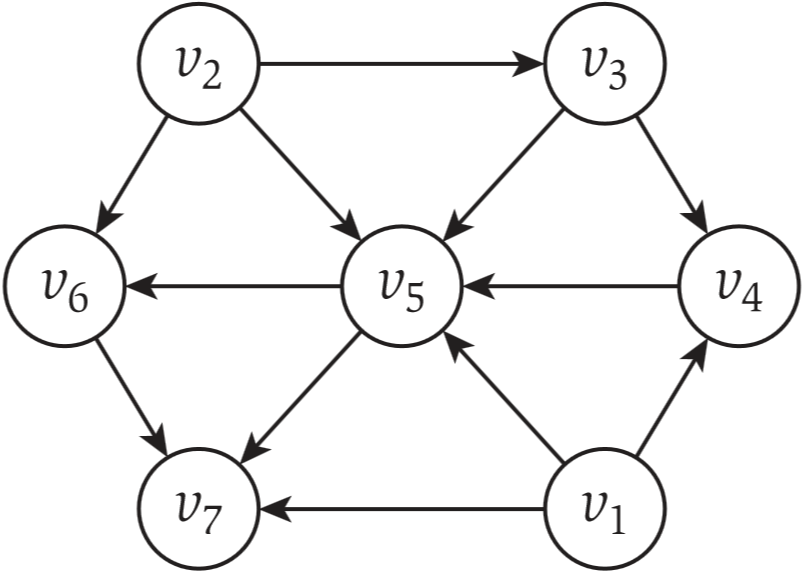
\includegraphics[width=0.45\linewidth]{img/dag}
	\end{figure}
	
\end{frame}



\begin{frame}{Ordenação topológica}

	\begin{itemize}
		\item \textbf{Problema:} dado um DAG, encontra uma ordem válida de processamento dos vértices, respeitando as precedências.
		\item \textbf{Ordem topológica:} uma ordenação dos vértices $v_1, v_2, \dots, v_n$ tal que para todo arco $(v_i, v_j)$, $i < j$.
		\begin{itemize}
			\item Ou seja, todos os arcos apontam para frente na ordenação.
			\item Exemplos: qual a ordem para cursar as disciplinas?
		\end{itemize}
	\end{itemize}


	\begin{figure}
		\centering
		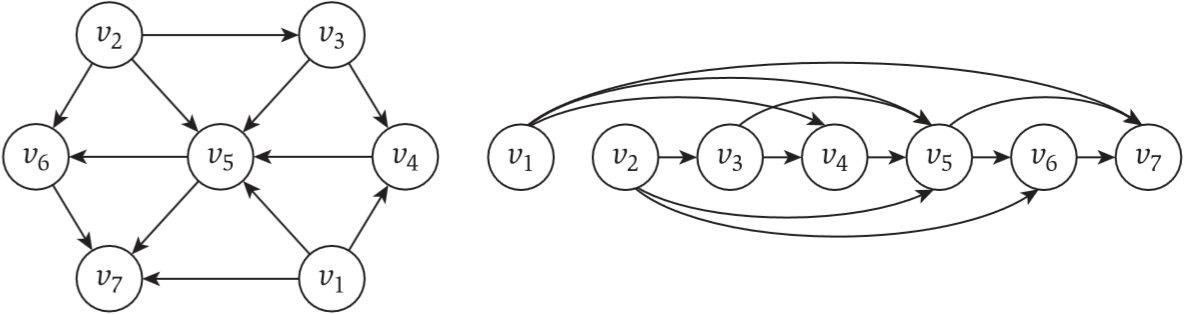
\includegraphics[width=0.9\linewidth]{img/ordenacao}
	\end{figure}
\end{frame}



\begin{frame}{Ordenação topológica}
	\framesubtitle{Propriedades}


	\begin{enumerate}
		\item $G$ possui uma ordenação topológica se e somente se $G$ é um DAG.
		\item Em todo DAG $G$, existe um vértice $v$ sem arcos incidentes.
	\end{enumerate}
	
	\pause
	
	\smallskip
	
	\textbf{Detalhes}
	
	\begin{itemize}
		\item Com relação à propriedade (1), existindo um ciclo, não é possível ordenar topologicamente seus vértices. Não existindo ciclo, é possível definir um primeiro vértice para a ordenação topológica e repetir o processo para os vértices restantes.
		
		\item Com relação à propriedade (2), caso todos os vértices tenham ao menos um arco incidente, necessariamente o grafo possui ao menos um ciclo e, consequentemente, não é um DAG.
	\end{itemize}
	
	\textbf{Exercício:} tente criar um DAGs que não respeitem as condições acima.
	
\end{frame}



\begin{frame}{Ordenação topológica}
	\framesubtitle{Algoritmo}
	
	\begin{algorithm}[H]
		\DontPrintSemicolon
		
		Find a vertex $v$ with no incoming arcs and order it first\;
		Delete $v$ from $G$\;
		Recursively compute a topological ordering of $G \setminus \{v\}$\;
		Append the result after $v$ and return the topological order.\;
		
		\caption{\texttt{topological-order(DAG G)}}
	\end{algorithm}
\end{frame}



\begin{frame}{Ordenação topológica}
	\framesubtitle{Funcionamento}

	\begin{figure}
		\centering
		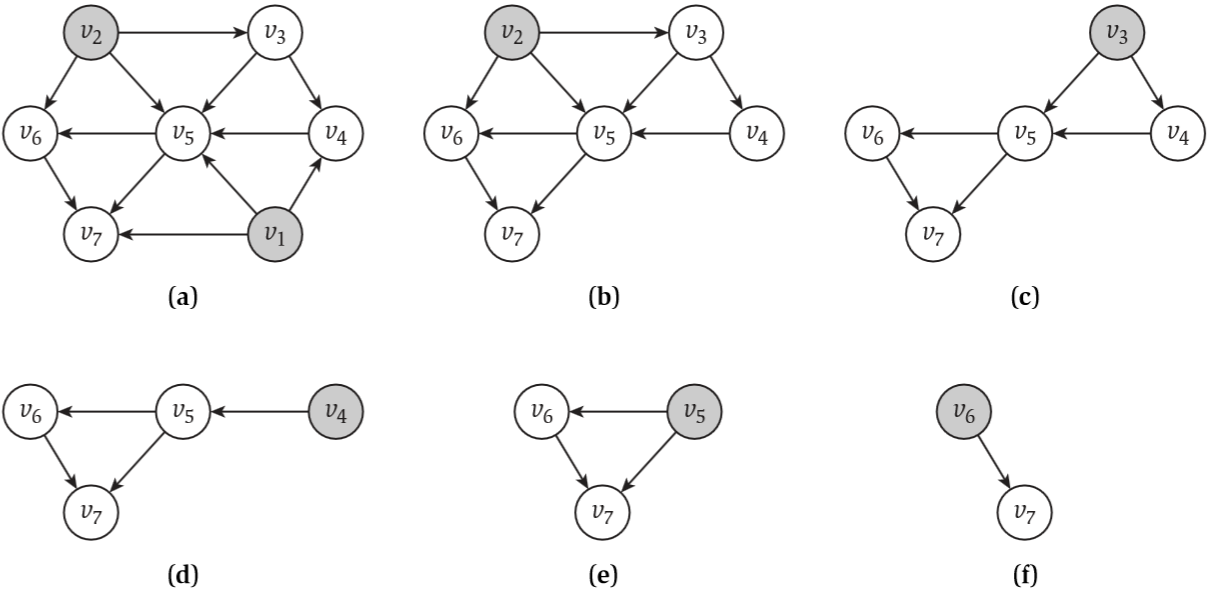
\includegraphics[width=1\linewidth]{img/execucao-ordenacao-topologica}
	\end{figure}

\end{frame}



\begin{frame}{Ordenação topológica}
	\framesubtitle{Complexidade}
	
	\begin{itemize}
		\item Encontrar o vértice $v$ demanda $O(n)$.
		\item O algoritmo executa $n$ iterações, totalizando $O(n^2)$.
		\item Para melhorar, fazemos a busca mais eficiente. Definimos um vértice ativo se ele ainda não foi deletados e mantemos:
		
		\begin{enumerate}
			\item Número de arcos incidentes para cada vértice a partir de vértices ativos.
			\item Vértices que não possuem arcos incidentes a partir de vértices ativos.
		\end{enumerate}
		
		\item No início, todos os vértices são ativos e a criação de (1) e (2) é feita com uma passagem sobre os vértices.
		
		\item A cada deleção do vértice $v$, percorremos todos os vértices $w$ para os quais $v$ possui arco, decrementando o valor em (1). Caso atinja zero, o vértice é incluído em (2).
		
		\item Logo, determinar um vértice sem arcos incidentes é feito em tempo constante.
		
		\item \textbf{Complexidade final:} $O(n + m)$.
	\end{itemize}
\end{frame}



\begin{frame}{Exercício}
	\framesubtitle{Ordenação topológica}
	
	\begin{enumerate}
		\item Crie um grafo com as disciplinas da matriz curricular do curso de Engenharia de Software, com as devidas relações de pré-requisitos. Implemente o algoritmo para determinação de ordenação topológica e calcule uma possível ordenação para cursar as disciplinas.
	\end{enumerate}
\end{frame}



\frame{
	\frametitle{Referências}	
	\setlength{\bibsep}{8pt plus 0.3ex}
	\fontsize{10pt}{10}\selectfont
	\bibliographystyle{apalike}
	\bibliography{../referencias}
}

\end{document}